%---- ENTRY 4
%
% This is the place where the proposed programme is to be described.
% This description is composed of two different sections.
%
% A) Scientific rationale: scientific background of the project,
% pertinent references; justification for present
% proposal.
%
% B) Immediate objective of the proposal: what specifically is to 
% be observed and what can be learnt from the observations so that 
% the feasibility becomes clear.
%

\smallskip
\noindent {\bf 2. Description of the proposed programme\\}
\noindent {\sl A) Scientific Rationale:}
\smallskip\\
Open clusters give one of the most relevant insights into both stellar and galactic evolution. Open clusters are classified as populations of sparsely bound stars.
The study of open clusters is done primarily by studying stellar populations by creating a colour-magnitude diagram (CMD). CMDs allow for the estimation of age, distance, metallicity, among other attributes of an open cluster. This is specifically done by the fitting of stellar isochrones, which are fitted to the CMD of the open cluster. Stellar isochrones are ways of fitting data on a CMD that allow the stellar evolutionary path to being determined directly from optical photometry, see \cite{1990BAAS...22.1288M} for a comprehensive example.  

 This has been shown to give accurate insight into both stellar and galactic evolution. \\  It has been shown by \cite{1980A&A....88..360V} that open clusters with an age of 1 Gyr are preferentially located on towards the galactic anti-centre. \cite{1950BAN....11...91O} found that there was an underabundance of old clusters relative to the number extrapolated by the population of their younger counterparts assuming uniform stellar formation rate throughout the galactic disk during its lifetime. \cite{1958ApJ...127...17S} deemed that the small number of old clusters was from disruptive interactions massive clouds towards the galactic core. However, the first large scale study of open clusters analysed by \cite{1988AJ.....95..771J} found that the disruptive processes were too efficient to support the population of the old breed of open clusters. Moreover, this first large scale analysis of the Lynga catalogue \citep{1982A&A...109..213L} found that the resultant cluster populations were determined through a nuanced relationship between inherent cluster properties, internal dynamics and overall environment in the galaxy. \\ Since then, Gaia has performed a large astrometric and photometric survey giving the first panoptic view of the galactic disk, which has allowed for a growth in catalogues like WEBDA. Studies such as \cite{2020A&A...640A...1C} have classified reddening, distance and age of $\sim$ 2000 clusters. Thus since many galactic tracing surveys have been completed, there has been a substantial improvement on the means to determine cluster parameters through isochrone fitting using supplementary high-resolution spectroscopic surveys such as \cite{Metallicity_catalogue} and \cite{2022MNRAS.509.1664J}. \\ Despite recent surveys, there are still many open clusters that lack sufficient cataloguing and parameters. This study proposes to study the position of open clusters in Milkey Way's disk and show how the inclusion of modern isochrone fitting can consolidate previous research in galactic tracing such as \cite{1982A&A...109..213L}. 
%-----
\begin{figure}[h!]
    \centering
    \subfloat[\centering Distance modulus against the log age of a sample of open-clusters.]{{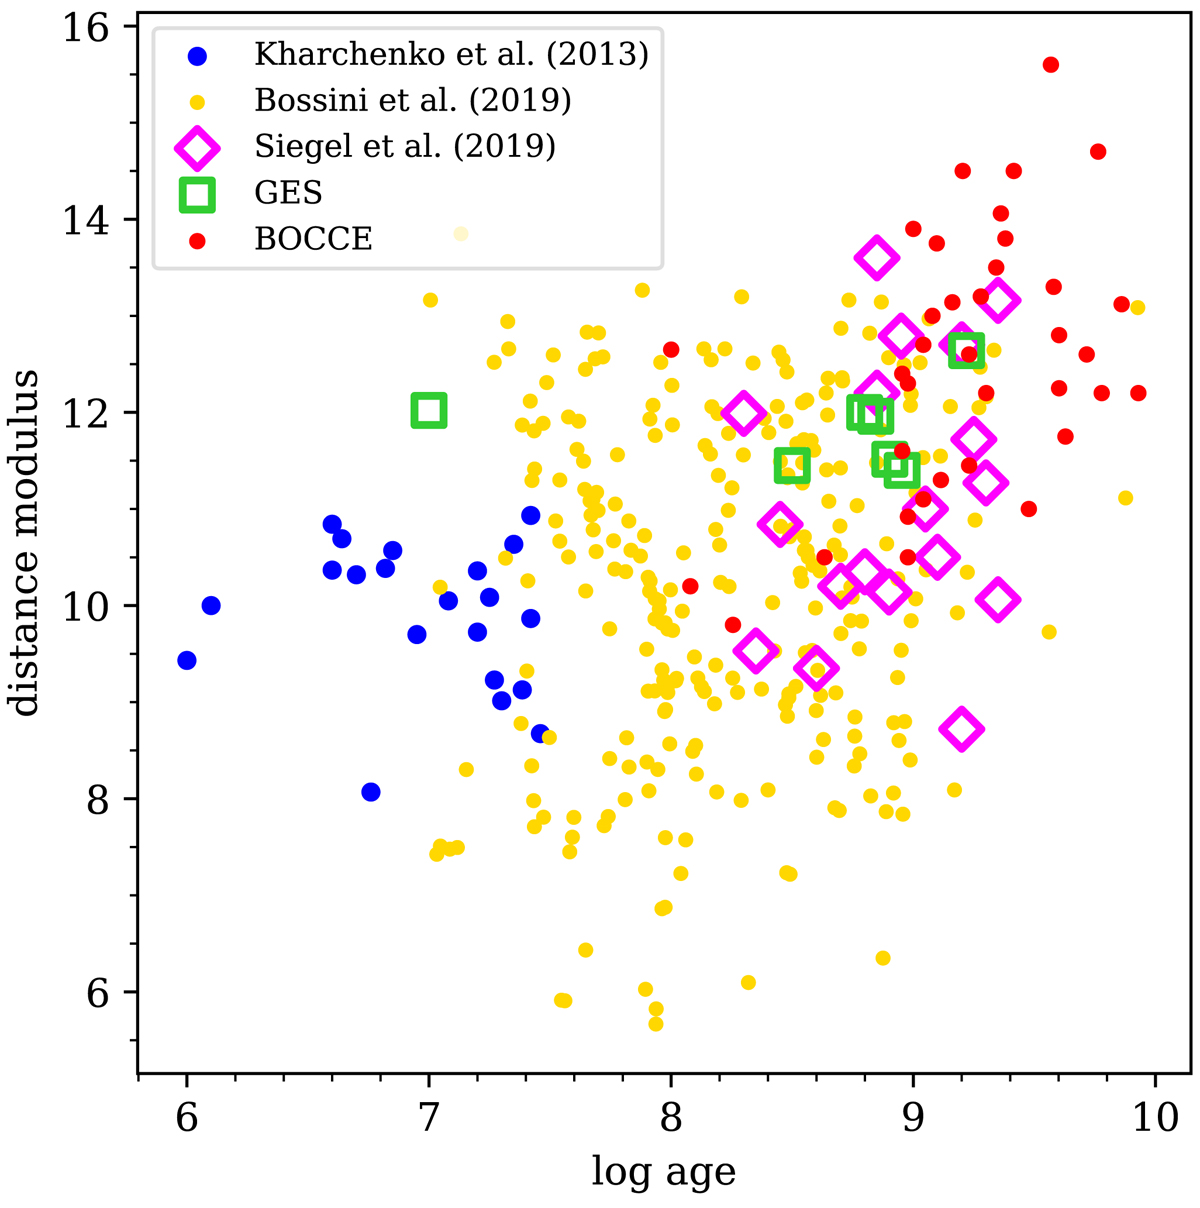
\includegraphics[width = 0.4\textwidth]{figs/aa38192-20-fig1.jpg}}}%
    \qquad
        \subfloat[\centering A comprehensive Hertzprung-Russell diagram which is colour-coded by cluster age.]{{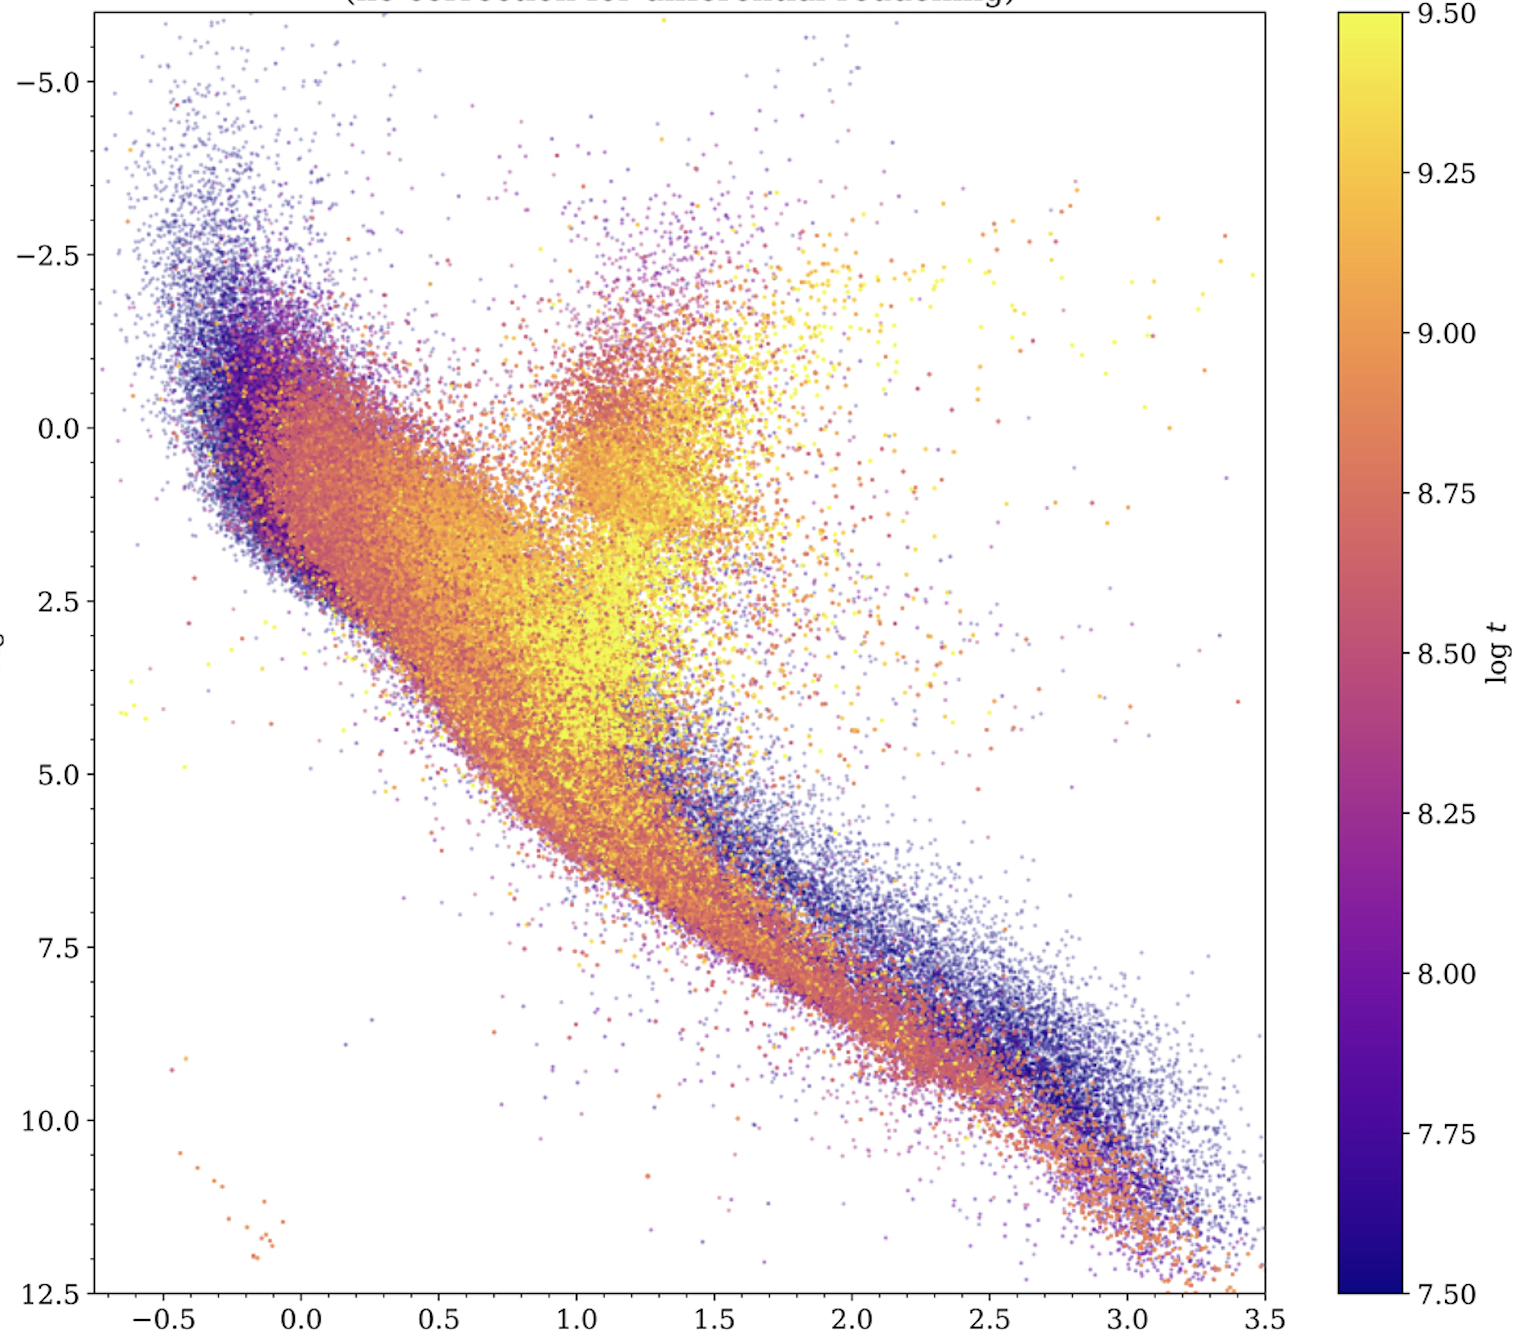
\includegraphics[width = 0.46\textwidth]{figs/Screenshot 2022-02-21 at 21.17.05.png}}}%
    \caption{Both plots provided by Galactic tracing study by \cite{2020A&A...640A...1C}.}%
    \label{fig:theory.}%
\end{figure}
%-----------------------------Figure End--------------------------------

\smallskip
\noindent {\sl B) Immediate Objective:}
\smallskip\\
The observation expedition proposes to observe a sample of open clusters from the WEBDA catalogue of varying ages and disk positions. This follows on from studies such as \cite{1982A&A...109..213L} and \cite{2004PASP..116..997V}. However, with the added advantage of using stellar isochrones from the MIST catalogue. These isochrones take full advantage of recent astrometric studies and improved isochrone models \citep[see.][]{2016ApJ...823..102C}. This allows parameters such as reddening, metalicity and convection overshooting to be estimated to a more satisfactory degree than prior studies of a similar nature. This includes things such as the oversight of convection overshooting when fitting isochrones as shown by \cite{2004PASP..116..997V}. Convection overshooting shows large discrepancies in the later stage of the main sequence. Correcting for this allows for cluster age to be interpolated at finer increments as a more reliable fit can be attained. 

Each cluster's stellar population will be analysed and classified based on the Trumpler system \citep{1930LicOB..14..154T}. This will be done by means of photometric analysis using \verb|photoutils| to create CMD plots for each cluster (\cref{fig:theory.} (b)). Following classification, a plot against distance age (\cref{fig:theory.} (a)) The distance of the cluster will be plotted against age to examine the abundance of older clusters on the outer disk and comment on the disruptive interactions with molecular clouds. Using provided CMD's, the presence of pre-main-sequence stars towards the galactic centre will examine. The main-sequence stage of intermediate aged clusters will also be examined. Following this, a comment on the interplay between age, distance and galactic environment can be postulated. Giving insight both into the shape of the milky way disk through tracing distance progression of clusters at varying ages. 
% State what specifically is to be observed and what can be learnt 
% from the observations, such that the feasibility becomes clear.

%
%---- ENTRY 5 ----------------------------------------------------------
%
% Provide a careful justification of the requested observing time,
% a feasibility study (expected signal-to-noise estimate 
% for the time requested; background estimates especially for extended 
% sources) and give information on the target visibility 
% 
% If proposing more than one target, indicate the priority. 
%
\smallskip
\noindent {\bf 3. Justification of requested observing time, 
feasibility and visibility}
\smallskip\\
This observation expedition proposes the observation of 12 open clusters of varying age. The clusters will be broken into three sets. Each set will comprise of 3 clusters of the following age categories, 'Young': age $<$ 200 Myr, 'Intermediate': 200 Myr $<$ age $<$ 1 Gyr and 'Old': 1 Gyr $<$ age. Each set will be observed at different areas of the galactic disk, see \cref{fig: mollweide_plot}. \\ A list of suitable targets with backup targets can be found in \cref{tb: targets}. \Cref{tb: targets} is organised by right ascension (RA) into groups (segregated) with varying ages in each RA window. A list of backup targets is also listed to be compatible with the corresponding group for the primary, and the study suggested if the main objective is not feasible. \\ Exposure time was selected to have a signal to noise ratio (SN) of $\sim$10 for the most feint members of a cluster population. However, doing this in some cases will cause either source to be saturated if bright or too noisy if feint. In this case, the exposure that adequately observed $\sim$98\% of the stellar population was chosen (\cref{fig: hist_plot}).
\begin{figure}[h!]
    \centering
    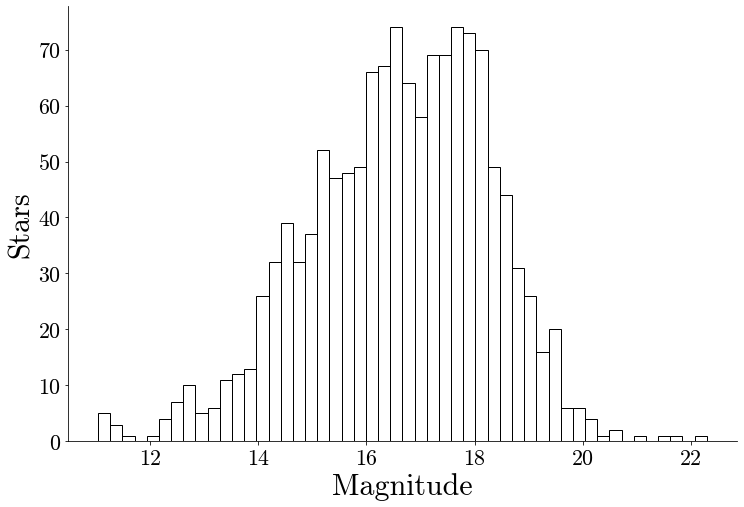
\includegraphics[width = 9cm]{figs/histogram.png}
    \caption{Example distribution of magnitude for stellar population of NGC2129}
    \label{fig: hist_plot}
\end{figure}



Each target will be observed in both \textbf{B} and \textbf{V} Johnson filters. As mentioned, each cluster will have SN $\simeq$10 for most feint members of the population. In turn, this provides an instrumental error on the magnitude of 0.1 or less. If inadequate samples from across the galactic disk are attained for a sufficient number of clusters, further numbers can be taken from archived data. In the case where the primary objective \textit{cannot} be completed, the observed data can be homogenised and used to catalogue membership and classification of each cluster, producing membership probability along with Trumpler classification of each cluster. This would provide cataloguing of poorly documented clusters see \cref{tb: targets}. As discussed with the use of MIST isochrones, ages, convections, and metalicities would be investigated to produce an elegant stellar catalogue for all observed clusters. This secondary objective would take a similar form to \cite{2004PASP..116..997V}.

\begin{figure}[h!]
    \centering
    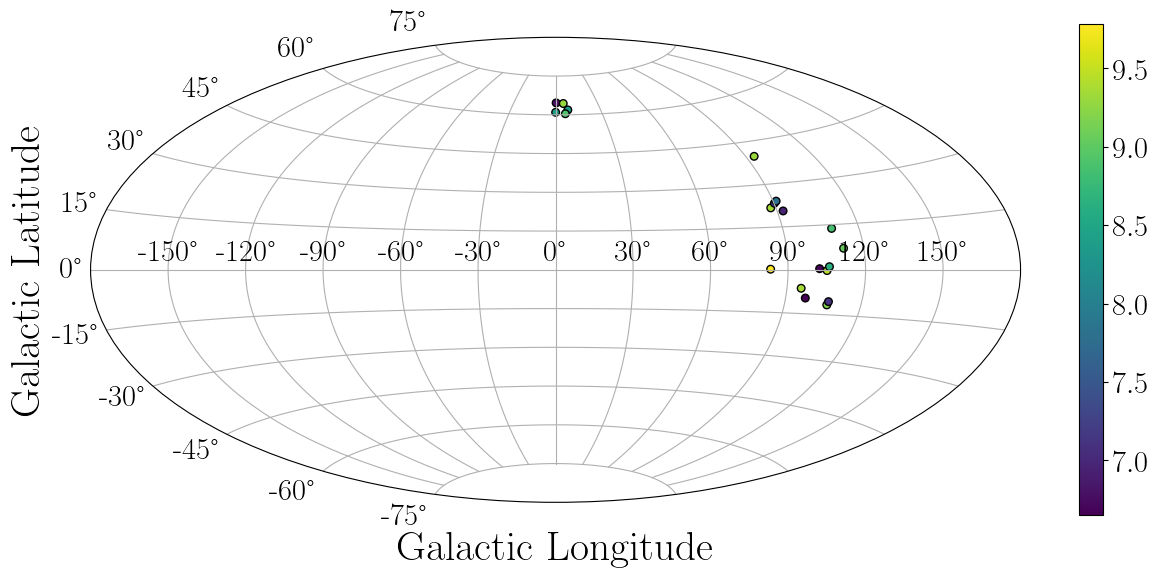
\includegraphics[width = 12cm]{figs/mollweide.png}
    \caption{Suggested open-cluster targets plotted in Galactic co-ordinates. Where the cluster age is shown using the color bar. Targets taken from the WEBDA database. }
    \label{fig: mollweide_plot}
\end{figure}

% Provide a careful justification of the requested observing time, a feasibility study (expected signal-to-noise estimate for the time requested...) and give information on the target visibility.
% If asking for more than one target, indicate the priority.
% Please do provide a list of back-up targets with coordinates, observing windows, time of transits (in the case of exoplanets) and exposures to use for each target. \textbf{You are allowed to have a table with backup targets in a 5th page}.



%
%---- ENTRY 6 ----------------------------------------------------------
% 
%
\pagebreak
\smallskip
\noindent {\bf 4. Previous/complementary data}\\ 
\noindent {\sl A) Preliminary Data:}
\smallskip\\
\cite{1982A&A...109..213L}\footnote{\url{https://heasarc.gsfc.nasa.gov/W3Browse/star-catalog/lyngaclust.html}} provided the first large scale database on open cluster it has all discussed parameters with specific bib information on where to find any missing parameters. WEBDA\footnote{\url{https://webda.physics.muni.cz/}} is an online version of the BDA created by \cite{1995ASSL..203..127M} it was the primary means of sourcing targets of it has collected most published data on open clusters with over 700 entries from the BDA and cross-references with other available catalogues. WEBDA provided all data seen in \cref{tb: targets}. SIMBAD\footnote{\url{http://simbad.u-strasbg.fr/simbad/}} was also used to cross-reference WEBDA during target selection process. 

\noindent {\sl B) Complementary Data:}
\smallskip\\
As there is no spectroscopic photometry performed or use of a U filter, the colour excess and the metalicity will need to be referenced. In the case of metalicity, the values will be inferred directly from observations through isochrones but will need to be supplemented by spectroscopic databases such as \cite{Metallicity_catalogue}. The second Gaia data release can be used for supporting astrometric data provided by studies such as \cite{2020A&A...640A...1C}. In the case where a larger sample size of clusters can give extra data, \cite{2022MNRAS.509.1664J} and \cite{2006A&A...446..121B}.

% \vfill

%Add here information about other data available to you that is relevant to the project and that it will be used in the final report. 
%Demonstrate that during the first semester and beginning of this semester, you have build the skills required to successfully complete the proposed project.

% Add here information about other data available to you that is relevant to the project and that it will be used in the final report. Mention what is the format of this data (are they magnitudes taken from a paper/database? are they images you need to analyse from the beginning? Include here how this data enhance your observations and how you will use it.